% ============================================================
% QSAR & Machine Learning Predictors - Teaching Slides
% Prepared for Chapter 6 (IQB JC Template)
% ============================================================

\documentclass[aspectratio=169,11pt]{beamer}

\usepackage{../theme/beamerthemeiqb}
\usepackage{../theme/iqb-layouts}
\renewcommand{\iqbheaderimage}{../theme/images/header.png}
\setstretch{1.05}

\usepackage{amsmath}
\usepackage{booktabs}
\usepackage{array}
\usepackage{tikz}
\usetikzlibrary{shapes,arrows,positioning,calc}

\title{Chapter 6: QSAR and Machine Learning Predictors}
\subtitle{From Foundational Concepts to Regulatory-Ready Models}
\author{Philipe Oliveira Fernandes \and Vinicius Gonçalves Maltarollo}
\institute{Graduate QSAR Workshop}
% \stuid{12207134}
% \major{生物物理学}
% \grade{直博四年级}
% \institute{生物物理研究所}
% \advisor{周如鸿 教授}
% \dateformat{zh}
\date{\today}
% Cover metadata for template cover
\papertitlechn{QSAR与机器学习预测器}
\papertitlechnsub{Chapter 6 教学幻灯片}
\paperengtitle{Chapter 6: QSAR and Machine Learning Predictors}

\begin{document}

% ============================================================
% Footer Configuration
% ============================================================
% Set footer style: left={default|custom}, center={section|title}, right={ratio|pageofy|zhpageofy}
\iqbfootline{default}{title}{pageofy}

% ------------------------------------------------------------
% 1. Cover
% ------------------------------------------------------------
\iqbcoverframe

% ------------------------------------------------------------
% Part 1: Fundamentals
% ------------------------------------------------------------
\iqbsectionframe{Fundamentals}{基础介绍}

% ------------------------------------------------------------
% 2. Chapter overview & learning goals
%  ------------------------------------------------------------
\begin{frame}{Chapter Map \& Learning Objectives}
  \iqblayouttwo{
    \iqbsectiontitle{Three learning goals}
    \begin{iqbitemize}
      \item Understand QSAR/QSPR theory and representation choices.
      \item Master modeling, validation, and OECD-aligned workflows.
      \item Scan emerging ML/GNN trends plus real-world deployment tips.
    \end{iqbitemize}

    \iqbsep

    \iqbsectiontitle{Scope of Chapter 6}
    \begin{iqbitemize}
      \item Descriptors \& fingerprints
      \item Classic vs. modern modeling
      \item OECD regulatory lens
      \item Validation, interpretation, applications, outlook
    \end{iqbitemize}
  }{
    \iqbsectiontitle{Lecture pacing (25 pages)}
    \begin{iqbitemize}
      \item Part 1: Fundamentals \& history (1--4)
      \item Part 2: Concepts \& representations (5--10)
      \item Part 3: OECD principles (11--13)
      \item Part 4: Software \& tools (14--15)
      \item Part 5: Validation \& controls (16--19)
      \item Part 6: Interpretation (20--21)
      \item Part 7: Practice \& cases (22--23)
      \item Part 8: Challenges \& summary (24--25)
    \end{iqbitemize}
  }
\end{frame}

% ------------------------------------------------------------
% 3. What is QSAR
% ------------------------------------------------------------
\begin{frame}{What is QSAR? Core Definitions}
  \iqblayouttwo{
    \iqbbluebox{Definition}{
      Quantitative Structure-Activity Relationship (QSAR) links molecular structure to measured
      biological activity or physicochemical property through mathematical models.
    }
    \iqbsep
    \begin{iqbitemize}
      \item Treats structure as descriptors/fingerprints and activity as endpoints.
      \item Serves as a rational design pillar in medicinal chemistry and chemical biology.
      \item Extends to QSPR, QSRR, QSTR depending on the endpoint class.
    \end{iqbitemize}
  }{
    \iqbsectiontitle{Why it matters}
    \begin{iqbitemize}
      \item Rapid hypothesis triage before synthesis or assays.
      \item Enables multi-parametric optimization (potency, ADME, toxicity).
      \item Bridges wet-lab measurements with ML-driven insights.
    \end{iqbitemize}

    \iqbsep

    \iqborangebox{Reminder}{
      QSAR quality is only as good as input structures, curated data, and validation discipline.
    }
  }
\end{frame}

% ------------------------------------------------------------
% 4. Historical background
% ------------------------------------------------------------
\begin{frame}{Historical Background \& Milestones}
  \iqblayouttwo{
    \begin{iqbitemize}
      \item 1863: Cros connects alcohol toxicity and solubility.
      \item 1884: Mills correlates melting/boiling points.
      \item 1962: Hansch equation formalizes multi-parameter QSAR.
      \item 1970s-1990s: Computer-assisted descriptors explode (logP, Hammett, 3D fields).
      \item 2000s: Regulatory guidance (OECD) codifies best practice.
      \item 2010s-2020s: ML/GNN and big data reshape predictive scope.
    \end{iqbitemize}
  }{
    \iqbsectiontitle{Naming evolution}
    \begin{iqbitemize}
      \item QSPR: structure-property (e.g., boiling point, solubility).
      \item QSRR: structure-reactivity (kinetics, catalysis).
      \item QSTR: structure-toxicity (safety profiling).
    \end{iqbitemize}

    \iqbgreenbox{Teaching cue}{
      Use timeline questions: ``Which inflection made QSAR mainstream?'' to recap Fig. 6.1 context.
    }
  }
\end{frame}

% ------------------------------------------------------------
% Frame A1: Hansch Equation (New Content)
% ------------------------------------------------------------
\begin{frame}{Hansch Equation: The Mathematical Foundation (1962)}
  \iqblayouttwo{
    \iqbsectiontitle{The Famous Equation}
    The Hansch equation relates biological activity to molecular descriptors:

    \[
    y = c_0 + c_1 X_1 + c_2 X_2 + \cdots + c_n X_n
    \]

    \begin{iqbitemize}
      \item $y$: biological activity (e.g., log(1/C), pIC$_{50}$)
      \item $X_i$: molecular descriptors (logP, $\sigma$, $E_s$, etc.)
      \item $c_i$: coefficients indicating descriptor importance
      \item Multi-parametric regression establishes structure-activity correlation
    \end{iqbitemize}
  }{
    \iqbsectiontitle{Historical Impact}
    \begin{iqbitemize}
      \item 1962: Hansch \& Fujita report on phenoxyacetic acids as plant growth regulators
      \item Introduced $\pi$ constant for hydrophobicity
      \item Pioneered quantitative approach to medicinal chemistry
      \item Foundation for all modern linear QSAR models
    \end{iqbitemize}

    \iqbsep

    \iqborangebox{Key Insight}{
      Coefficients reveal \textit{how} and \textit{how much} each structural feature modulates activity
    }
  }
\end{frame}

% ------------------------------------------------------------
% Frame A2: Data Quality & Structure Curation
% ------------------------------------------------------------
\begin{frame}{Data Quality: ``Trust, but Verify'' (OECD P1)}
  \iqblayouttwo{
    \iqbsectiontitle{Why Data Curation Matters}
    \begin{iqbitemize}
      \item \textbf{Bad data $\Rightarrow$ Bad model} (garbage in, garbage out)
      \item Outliers, duplicates, and measurement errors skew statistics
      \item Structural ambiguity: tautomers, stereoisomers, protonation states
      \item OECD Principle 1: Experimental values must be reliable
    \end{iqbitemize}

    \iqbsep

    \iqbgreenbox{Data Cleaning Pipeline}{
      Detect outliers (Z-score, IQR) $\rightarrow$ Normalize scales $\rightarrow$ Verify structures $\rightarrow$ Remove/flag duplicates
    }
  }{
    \iqbsectiontitle{Quality Indicators}
    \begin{iqbitemize}
      \item \textbf{Measurement error}: Assay CV, detection limit
      \item \textbf{Structural confidence}: X-ray vs. computational; validated tautomer set
      \item \textbf{Activity range}: Log-scale variation (e.g., pIC$_{50}$ 4--10)
      \item \textbf{Temporal consistency}: Same assay protocol over time
    \end{iqbitemize}

    \iqbsep

    \iqborangebox{OECD Connection}{
      OECD P1 codifies these principles in regulatory QSAR guidance for hazard assessment
    }
  }
\end{frame}

% ------------------------------------------------------------
% Frame A3: Regression Metrics (Linear QSAR)
% ------------------------------------------------------------
\begin{frame}{Regression Metrics: Goodness-of-Fit \& Predictivity}
  \iqblayoutthree{
    \iqbsectiontitle{Fitting Metrics}
    \iqbsep
    \textbf{R$^2$ (R-squared):}
    \[
    R^2 = 1 - \frac{\sum(y_i - \hat{y}_i)^2}{\sum(y_i - \bar{y})^2}
    \]
    Fit to training data; risk of overfitting.

    \textbf{Q$^2$ (Cross-validated):}
    \[
    Q^2 = 1 - \frac{\sum(y_i - \hat{y}_i)^2_{CV}}{\sum(y_i - \bar{y})^2}
    \]
    Leave-One-Out (LOO) or 5-fold CV.
  }{
    \iqbsectiontitle{Predictivity Metrics}
    \iqbsep
    \textbf{Golbraikh--Tropsha Criteria:}
    \begin{enumerate}
      \item $Q^2 > 0.5$
      \item $R^2 - Q^2 < 0.3$
      \item $R_m^2 = r^2(1-\sqrt{|r^2-r_0^2|})$
      \item $|r_0^2 - r'^2_0| < 0.3$
    \end{enumerate}
    Ensures not just lucky fit.
  }{
    \iqbsectiontitle{External Validation}
    \iqbsep
    \textbf{Test Set Q$^2_F$:}
    \[
    Q^2_F = 1 - \frac{\sum(y_i - \hat{y}_i)^2_{test}}{\sum(y_i - \bar{y}_{train})^2}
    \]
    On completely held-out data.

    \iqbsep

    \textbf{CCC (Concordance):} Bland--Altman plot; agreement ratio $\geq 0.85$.
  }
\end{frame}

% ------------------------------------------------------------
% Frame A4: Classification Metrics (Binary QSAR)
% ------------------------------------------------------------
\begin{frame}{Classification Metrics: Beyond Accuracy}
  \iqblayouttwo{
    \iqbsectiontitle{Confusion Matrix \& Derived Metrics}
    \iqbsep
    \begin{tabular}{|c|cc|}
      \hline
      & \textbf{Pred+} & \textbf{Pred-} \\
      \hline
      \textbf{True+} & TP & FN \\
      \textbf{True-} & FP & TN \\
      \hline
    \end{tabular}

    \iqbsep

    \begin{iqbitemize}
      \item \textbf{Sensitivity} = $\frac{\text{TP}}{\text{TP}+\text{FN}}$ (recall)
      \item \textbf{Specificity} = $\frac{\text{TN}}{\text{TN}+\text{FP}}$
      \item \textbf{Precision} = $\frac{\text{TP}}{\text{TP}+\text{FP}}$
      \item \textbf{F1} = $\frac{2 \cdot \text{Prec} \cdot \text{Rec}}{\text{Prec} + \text{Rec}}$
    \end{iqbitemize}
  }{
    \iqbsectiontitle{Advanced Metrics}
    \small
    \begin{iqbitemize}
      \item \textbf{MCC} (Matthews Corr. Coef.) \\
            $\text{MCC} = \frac{\text{TP} \cdot \text{TN} - \text{FP} \cdot \text{FN}}{\sqrt{(\text{TP}+\text{FP})(\text{TP}+\text{FN})(\text{TN}+\text{FP})(\text{TN}+\text{FN})}}$\\[0.1cm]
            Balanced, handles imbalanced data.

      \item \textbf{ROC--AUC}: Sensitivity vs. (1-Specificity) curve; AUC = 0.5 (random), 1.0 (perfect).

      \item \textbf{Enrichment Factor} (EF) for screening: \\
            $\text{EF} = \frac{\text{\% actives in top 10\%}}{\text{\% actives overall}}$
    \end{iqbitemize}
  }
\end{frame}

% ------------------------------------------------------------
% Frame A5: Y-Scrambling & X-Scrambling (Validation)
% ------------------------------------------------------------
\begin{frame}{Y-Scrambling \& X-Scrambling: Testing Model Robustness}
  \iqblayouttwo{
    \iqbsectiontitle{Y-Scrambling (Activity)}

    Randomly permute the response variable $y$ while keeping $X$ fixed. Refit the model.

    \begin{iqbitemize}
      \item \textbf{Expected:} Q$^2$ near 0, R$^2$ high
      \item \textbf{False positive:} If Q$^2_{scrambled} \approx Q^2_{orig}$ $\Rightarrow$ test fails
      \item \textbf{Overfitting:} If R$^2_{scrambled} > 0.3$ $\Rightarrow$ alarm
      \item \textbf{Protocol:} Repeat 100--1000 times; plot
    \end{iqbitemize}

    \iqbgreenbox{Key Output}{
      Y-scrambling prevents claiming predictive power from random coincidence
    }
  }{
    \iqbsectiontitle{X-Scrambling (Descriptor)}
    Randomize descriptor columns; keep $y$ correct. Refit.

    \begin{iqbitemize}
      \item[For classification] Q$^2$ and MCC should collapse
      \item Detects multicollinearity artifacts
      \item Shows if model relies on noise
      \item Progressive corruption of features
    \end{iqbitemize}

    \iqbsep

    \iqborangebox{Statistical Test}{
      \% scrambled $\ll 5\%$ at $p=0.05$
    }
  }\end{frame}

% ------------------------------------------------------------
% Frame A6: Applicability Domain (Defining Model Limits)
% ------------------------------------------------------------
\begin{frame}{Applicability Domain (AD): Where Does the Model Work?}
  \frametitle[Applicability Domain]{Applicability Domain (AD): Where Does the Model Work?}
\iqblayoutthree{
    \iqbsectiontitle{Range-Based (Simplest)}
    \small
    Min--max boundaries on each descriptor.

    \iqbsubsectiontitle{Pro} Fast, interpretable

    \iqbsubsectiontitle[red]{Con} Ignores multivariate structure

    Example: logP $\in [1,5]$, TPSA $\in [20,120]$ Å$^2$
  }{
    \iqbsectiontitle{Distance-Based (PCA/Leverage)}
    \small
    Compounds far from training set center (Mahalanobis, leverage $> h_{crit}$) are outside AD.

    \iqbsubsectiontitle{Pro} Accounts for correlation

    \iqbsubsectiontitle[red]{Con} Sensitive to outliers; assumes linear manifold

    Leverage: $h_i = \mathbf{x}_i (\mathbf{X}^T\mathbf{X})^{-1}\mathbf{x}_i^T$
  }{
    \iqbsectiontitle{Probability Density Methods}
    \small
    KDE, Gaussian mixture, or kernel density in descriptor space.

    \iqbsubsectiontitle{Pro} Flexible; multi-modal support

    \iqbsubsectiontitle[red]{Con} Computationally heavier; threshold subjective

    $p(\mathbf{x}) = \frac{1}{n} \sum_i K(\mathbf{x} - \mathbf{x}_i)$
  }
\end{frame}

% ------------------------------------------------------------
% Part 2: Core Concepts
% ------------------------------------------------------------
\iqbsectionframe{Core Concepts}{核心概念}

% ------------------------------------------------------------
% 5. QSAR workflow
% ------------------------------------------------------------
\begin{frame}{QSAR Modeling Workflow (Fig. 6.1 Inspired)}
  \iqblayouttwo{
    \iqbsectiontitle{Four canonical steps}
    \begin{enumerate}
      \item \textbf{Data acquisition \& curation}\\
            Gather endpoints, harmonize assays, deduplicate, verify structures.
      \item \textbf{Molecular representation}\\
            Choose descriptors/fingerprints/graphs; consider protonation and tautomers.
      \item \textbf{Modeling}\\
            Linear (MLR/PLS) or nonlinear (SVM, RF, DL); document hyperparameters.
      \item \textbf{Training/test protocol}\\
            Split strategies, internal validation loops, independent external sets.
    \end{enumerate}
  }{
    \iqbsectiontitle{Quality checkpoints}
    \begin{iqbitemize}
      \item Structure standardization (Fourches et al. ``Trust, but verify'').
      \item Endpoint alignment: same units, biological context, experimental variance.
      \item Metadata logging for reproducibility (software versions, seeds, splits).
      \item Visual inspection: Fig. 6.1 pipeline as classroom walk-through.
    \end{iqbitemize}
  }
\end{frame}

% ------------------------------------------------------------
% 6. Descriptor taxonomy
% ------------------------------------------------------------
\begin{frame}{Molecular Descriptors: 1D to 6D}
  \footnotesize
  \begin{tabular}{p{0.08\textwidth}p{0.28\textwidth}p{0.52\textwidth}}
    \toprule
    Dim & Definition & Representative features and notes\\
    \midrule
    1D & Scalar counts & Atom counts, bonds, rings, heteroatoms. Fast, coarse.\\
    2D & Topological & Connectivity indices, Kier--Hall, fragment counts, logP. Captures adjacency.\\
    3D & Shape/conformation & Steric/electrostatic fields, CoMFA grids, distances. Needs aligned 3D structures.\\
    4D & Multiple conformations & Ensemble averaged descriptors; solvent/excitation snapshots.\\
    5D & Environmental sampling & Explicit receptor/protein interactions or multiple alignment hypotheses.\\
    6D & Dynamic conditions & Time-dependent properties, induced fit, environmental perturbations.\\
    \bottomrule
  \end{tabular}

  \iqbsep
  \begin{iqbitemize}
    \item Higher dimensions capture richer physics but demand more sampling and validation.
    \item Use Fig. 6.2 narratives to highlight when 3D+ is justified (e.g., binding pocket specificity).
  \end{iqbitemize}
\end{frame}

% Frame G1: Descriptor Types (Constitutional, Topological, etc.)
\begin{frame}{Five Descriptor Types: What Each Captures}
  \iqblayoutthree{
    \iqbsectiontitle{Constitutional}
    Molecular formula, atom counts, heteroatom types.

    \iqbsep

    \iqbsubsectiontitle{Example}
    \# C atoms, \# H-bonds, MW, \# rotatable bonds

    \iqbsep

    \iqbbluebox{Nature}{No connectivity info; fastest}
  }{
    \iqbsectiontitle{Topological}
    Connectivity between atoms; graph properties.

    \iqbsep

    \iqbsubsectiontitle{Example}
    Kier--Hall, Randić indices, SMILES-derived patterns

    \iqbsep

    \iqbbluebox{Nature}{2D structure; captures neighborhood}
  }{
    \iqbsectiontitle{Geometrical}
    3D spatial arrangement; distances, angles, surface area.

    \iqbsep

    \iqbsubsectiontitle{Example}
    TPSA, Moment of inertia, van der Waals volume

    \iqbsep

    \iqbbluebox{Nature}{3D structure; alignment-dependent}
  }
\end{frame}

% Frame G2: Electronic & Thermodynamic Descriptors
\begin{frame}{Electronic \& Thermodynamic Descriptors}
  \iqblayouttwo{
    \iqbsectiontitle{Electronic}
    Orbital energies, partial charges, polarizability, HOMO/LUMO gaps.

    \iqbsep

    \iqbsubsectiontitle{Examples}
    \begin{iqbitemize}
      \item Mulliken/Gasteiger partial charges
      \item Quantum chemical descriptors (DFT-derived)
      \item Electronegativity sums
    \end{iqbitemize}

    \iqbsep

    \iqbbluebox{Pros}{Mechanistically meaningful}

    \iqbbluebox{Cons}{Computationally expensive}
  }{
    \iqbsectiontitle{Thermodynamic}
    Enthalpy, free energy, solvation energy contributions.

    \iqbsep

    \textbf{Application:}
    \begin{iqbitemize}
      \item QSPR for solubility, melting point
      \item ADME predictions
      \item Binding affinity estimation
    \end{iqbitemize}

    \iqbsep

    \iqbbluebox{Challenge}{Requires MD sampling or QM calculations}
  }
\end{frame}

% ----------- -------------------------------------------------------
% 7. Fingerprints
% ------------------------------------------------------------
\begin{frame}{Molecular Fingerprints \& Vector Encodings}
  \iqblayouttwo{
    \iqbsectiontitle{Concept}
    \begin{iqbitemize}
      \item Bit strings or count vectors derived from atom neighborhoods.
      \item Examples: MACCS, ECFP/FCFP, MHFP, pharmacophore keys.
      \item Encode presence/absence of substructures for fast similarity search.
    \end{iqbitemize}

    \iqbsep

    \iqborangebox{Design choices}{
      Radius/diameter, hashing length, folded vs. unfolded vectors, chirality toggles.
    }
  }{
    \iqbsectiontitle{Teaching tips}
    \begin{iqbitemize}
      \item Contrast with descriptors: fingerprints are sparse binary, descriptors are engineered scalars.
      \item Relate to Fig. 6.2(b): show how fragments map onto specific bit positions.
      \item Demonstrate Tanimoto similarity and collision issues for hashed fingerprints.
    \end{iqbitemize}
  }
\end{frame}

% ------------------------------------------------------------
% 8. Traditional QSAR methods
% ------------------------------------------------------------
\begin{frame}{Traditional 3D-QSAR Families: CoMFA, CoMSIA, HQSAR}
  \iqblayouttwo{
    \iqbsectiontitle{CoMFA \& CoMSIA}
    Grid-based MIF methods.

    \iqbsep

    \begin{iqbitemize}[1.5cm]
      \item[CoMFA] Steric + E-static fields; requires alignment
      \item[CoMSIA] Gaussian indices; more robust
      \item Both use PLS; great for congenerics
    \end{iqbitemize}
 
    \iqbsep

    \iqbsectiontitle{HQSAR}
    Fragment-based; no 3D alignment. Diverse scaffolds.
  }{
    \iqbimgcenter[width=0.9\textwidth]{images/qsar-ml-chap6/6.3.png}
  }
\end{frame}

% ------------------------------------------------------------
% Frame B1: 3D-QSAR Methods Detailed Comparison
% ------------------------------------------------------------
\begin{frame}{CoMFA vs. CoMSIA vs. HQSAR: In-Depth Comparison}
  \frametitle[CoMFA vs. CoMSIA vs. HQSAR]{CoMFA vs. CoMSIA vs. HQSAR: In-Depth Comparison}
\small
  \begin{tabular}{|l|ccc|}
    \hline
    \textbf{Criterion} & \textbf{CoMFA} & \textbf{CoMSIA} & \textbf{HQSAR} \\
    \hline
    \textbf{Alignment dependency} & High & Medium & None \\
    \textbf{Grid-based?} & Yes & Yes & No (hologram) \\
    \textbf{Descriptors} & Steric, E-static & 5 GRID fields & Fragment hashes \\
    \textbf{Congeneric series} & Excellent & Very good & Good \\
    \textbf{Diverse scaffolds} & Weak & Medium & Excellent \\
    \textbf{Interpretability} & Contour maps & Field maps & Atom binning \\
    \textbf{Robustness to noise} & Lower & Higher & Higher \\
    \textbf{3D structure need} & Full 3D & Full 3D & Only scaffold \\
    \hline
  \end{tabular}

  \iqbsep

  \iqbgreenbox{Practical Guide}{
    Start with HQSAR for rapid screening of diverse libraries. Use CoMSIA for congeneric SAR optimization to avoid alignment pitfalls. CoMFA remains gold standard for legacy projects with well-aligned analogs.
  }
\end{frame}

% ------------------------------------------------------------
% Frame B2: Rational Data Splitting Strategies
% ------------------------------------------------------------
\begin{frame}{Rational Train/Test Splitting: Beyond Random Shuffle}
  \frametitle[Train/Test Splitting]{Rational Train/Test Splitting: Beyond Random Shuffle}
\iqblayouttwo{
    \iqbsectiontitle{Why Splitting Matters}
    \small
    \begin{iqbitemize}
      \item \textbf{Random split}: Unbiased but may group similar compounds into same set
      \item \textbf{Temporal split}: First 70\% training, last 30\% test (realistic deployment scenario)
      \item \textbf{Diversity-based}: Use TMAP/t-SNE to split dissimilar compounds into train/test
      \item \textbf{Stratified}: Maintain activity distribution balance in both sets
    \end{iqbitemize}

    \iqbsep

    \iqborangebox{Example: Stratified K-Fold}{
      Ensure each fold contains proportional active/inactive compounds; prevents fate of imbalanced classes
    }
  }{
    \iqbsectiontitle{Algorithm: Hierarchical Splitting}
    \small
    1. Compute Tanimoto/Euclidean distances on fingerprints/descriptors

    \iqbsep

    2. Use hierarchical clustering $\rightarrow$ prune at threshold to get $k$ clusters

    \iqbsep

    3. Randomly sample compounds from each cluster proportionally into train/test

    \iqbsep

    4. Verify: no cluster $> 80\%$ in training set

    \iqbsep

    \iqbgreenbox{Statistical Test}{
      Chi-square test: descriptor distributions train vs. test should be $p > 0.05$
    }
  }\end{frame}

% ------------------------------------------------------------
% 9. Modern ML
% ------------------------------------------------------------
\begin{frame}{Modern Machine Learning in QSAR}
  \iqblayouttwo{
    \iqbsectiontitle{Why ML gained traction}
    \begin{iqbitemize}
      \item Handles nonlinearity, multi-task targets, and high-dimensional descriptors.
      \item Data abundance (ChEMBL, PubChem) plus open-source toolkits (RDKit, scikit-learn).
      \item GPU-accelerated deep learning shortens iteration cycles.
    \end{iqbitemize}
  }{
    \iqbsectiontitle{Model zoo}
    \begin{iqbitemize}
      \item Ensemble trees: Random Forest, XGBoost for tabular descriptors.
      \item Kernel methods: SVM, Gaussian Process for smaller data.
      \item Neural nets: FCNN, CNN on SMILES, sequence transformers.
      \item Self-supervised encoders + transfer learning for scarce endpoints.
    \end{iqbitemize}
  }
\end{frame}

% ------------------------------------------------------------
% 10. Graph learning
% ------------------------------------------------------------
\begin{frame}{Molecular Graphs \& GNN Pipelines (cf. Fig. 6.5)}
  \iqblayouttwo{
    \iqbsectiontitle{Graph construction}
    \begin{iqbitemize}
      \item Nodes: atom types, charges, aromaticity, hybridization, 3D coordinates.
      \item Edges: bond order, conjugation, ring membership, spatial distances.
      \item Optional 3D info via message passing with distance/angle encodings.
    \end{iqbitemize}

    \iqbsep

    \iqborangebox{Preprocessing reminders}{
      Standardize valence, add explicit hydrogens when needed, keep conformer IDs for 3D GNNs.
    }
  }{
    \iqbsectiontitle{Representative models}
    \begin{iqbitemize}
      \item Chemprop message passing network (MPNN) for activity prediction.
      \item Graph attention (GAT), GraphConv, DimeNet, SchNet for 3D-aware tasks.
      \item Multi-task heads for simultaneous potency, ADME, toxicity endpoints.
    \end{iqbitemize}
  }
\end{frame}

% ------------------------------------------------------------
% Part 3: OECD Principles
% ------------------------------------------------------------
\iqbsectionframe{OECD Principles}{OECD原则}

% ------------------------------------------------------------
% 11. OECD overview - TEMPORARILY DISABLED FOR DEBUGGING
% ------------------------------------------------------------
% \begin{frame}{OECD Principles Overview (Regulatory Lens)}
%   \iqblayouttwo{
%     \iqbsectiontitle{Why OECD matters}
%     \begin{iqbitemize}
%       \item Provides transparent criteria for accepting QSARs in regulatory submissions.
%       \item Aligns academic best practices with industrial risk management.
%       \item Drives reproducibility, documentation, and interpretability expectations.
%     \end{iqbitemize}
%   }{
%     \iqbgreenbox{Five principles snapshot}{
%       \begin{enumerate}
%         \item Defined endpoint.
%         \item Unambiguous algorithm.
%         \item Defined applicability domain (AD).
%         \item Goodness-of-fit, robustness, predictivity metrics.
%         \item Mechanistic interpretation where possible.
%       \end{enumerate}
%     }}
% \end{frame}

% ------------------------------------------------------------
% 12. OECD 1-3
% ------------------------------------------------------------
\begin{frame}{OECD Principles 1-3: Practical Notes}
  \iqblayouttwo{
    \iqbsectiontitle{P1. Defined endpoint}
    \begin{iqbitemize}
      \item Detail assay type, organism, conditions, units, variance.
      \item Ensure consensus across merged datasets; flag outliers.
    \end{iqbitemize}
    \iqbsep
    
    \iqbsectiontitle{P2. Unambiguous algorithm}
    \begin{iqbitemize}
      \item Document software versions, equations, hyperparameters.
      \item Clarify randomness control (seeds) and feature engineering steps.
    \end{iqbitemize}
  }{
    \iqbsectiontitle{P3. Applicability domain}
    \begin{iqbitemize}
      \item Define AD strategy (distance to training set, leverage, probability density).
      \item Label predictions as reliable/uncertain based on AD score.
      \item Discuss AD limitations during interpretation to manage risk.
    \end{iqbitemize}
  }
\end{frame}

% ------------------------------------------------------------
% 13. OECD 4-5
% ------------------------------------------------------------
\begin{frame}{OECD Principles 4-5: Validation \& Mechanism}
  \iqblayouttwo{
    \iqbsectiontitle{P4. Statistical performance}
    \begin{iqbitemize}
      \item Report internal (CV) and external metrics (see frames 17-18).
      \item Avoid overfitting: compare training vs. validation trends, use Y-randomization checks.
      \item Provide uncertainty estimates (confidence intervals, bootstraps).
    \end{iqbitemize}
  }{
    \iqbsectiontitle{P5. Mechanistic interpretation}
    \begin{iqbitemize}
      \item Link model features to known SAR insights or physicochemical rationale.
      \item Discuss when mechanism is not feasible (novel targets, purely statistical models).
      \item Use contour maps, feature attribution, or experimental follow-up to strengthen claims.
    \end{iqbitemize}
  }
\end{frame}

% ------------------------------------------------------------
% Part 4: Software & Tools
% ------------------------------------------------------------
\iqbsectionframe{Software and Tools}{软件工具}

% ------------------------------------------------------------
% 14. Descriptor tools
% ------------------------------------------------------------
\begin{frame}{Descriptor Calculation Tools \& Data Sources}
  \footnotesize
  \begin{tabular}{p{0.18\textwidth}p{0.35\textwidth}p{0.32\textwidth}}
    \toprule
    Tool & Coverage & Teaching notes\\
    \midrule
    Dragon & \(>5000\) descriptors (1D-3D) & Commercial benchmark, good for comparison studies.\\
    PaDEL-Descriptor & 1D-3D + fingerprints & Free, GUI/CLI, integrates CDK features.\\
    RDKit & Custom features, fingerprints & Python/C++; reproducible pipelines with notebooks.\\
    Mordred & 1800+ descriptors & Scriptable via Python, easy to extend.\\
    alvaDesc, ChemDes & Cloud/calculator hybrids & Useful for quick prototypes.\\
    \bottomrule
  \end{tabular}

  \iqbsep
  \iqbbluebox{Data inflow}{
    ChEMBL, PubChem, BindingDB, PDBbind feed curated endpoints. Normalize units and assay notes before descriptor generation.
  }
\end{frame}

% Frame D1: Public Benchmarks & Datasets
\begin{frame}{Open Datasets \& Benchmarking (Reproducibility)}
  \iqblayouttwo{
    \iqbsectiontitle{Gold-standard datasets}
    \begin{iqbitemize}
      \item \textbf{CHEMBL24+}: 2M+ activity records; curated, standardized
      \item \textbf{PubChem}: Millions; variable quality but searchable
      \item \textbf{PDBbind}: Binding affinity; crystal structure PDB IDs
      \item \textbf{MolNet}: Assembled benchmarks for regression/classification
    \end{iqbitemize}

    \iqbsep

    \iqbgreenbox{Why public?}{
      Enables direct model comparison; boosts reproducibility and trust
    }
  }{
    \iqbsectiontitle{Benchmark protocols}
    \small
    \begin{iqbitemize}
      \item \textbf{Leaderboards:} SAMPL challenges, MoleculeNet rankings, RegioSQM.
      \item \textbf{To evaluate:} Robustness to data splits, generalization, interpretation stability.
    \end{iqbitemize}
  }
\end{frame}

% Frame D2: Industrial Deployment Lessons
\begin{frame}{Moving QSAR to Production: Real-World Lessons}
  \iqblayoutthree{
    \iqbsectiontitle{Early stages}
    \small
    \begin{iqbitemize}
      \item Validate on internal projects before \textit{de novo}
      \item Cross-functional sign-off (chemists, biologists)
      \item Document assumptions; flag edge cases
    \end{iqbitemize}
  }{
    \iqbsectiontitle{Scaling phase}
    \small
    \begin{iqbitemize}
      \item Continuous retraining on new data
      \item A/B test: ML vs. human prioritization
      \item Monitor prediction confidence; flag AD violations
    \end{iqbitemize}
  }{
    \iqbsectiontitle{Maintenance}
    \small
    \begin{iqbitemize}
      \item Retrain quarterly; version control models
      \item Track hit rates, false positives
      \item User feedback loop
      \item Explainability == trust
    \end{iqbitemize}
  }
\end{frame}

% ------------------------------------------------------------
% 15. QSAR platforms
% ------------------------------------------------------------
\begin{frame}{QSAR Modeling Platforms \& Software Ecosystem}
  \iqblayouttwo{
    \iqbsectiontitle{Programming-centric stack}
    \begin{iqbitemize}
      \item RDKit + scikit-learn / PyTorch / TensorFlow.
      \item DeepChem, OpenFF, ADMETlab APIs.
      \item TeachOpenCADD notebooks for instructional demos.
    \end{iqbitemize}
    \iqbsep
    \iqbsectiontitle{Why scripting?}
    \begin{iqbitemize}
      \item Full transparency, version control, automation for benchmarking.
      \item Easier integration with lab notebooks and LIMS.
    \end{iqbitemize}
  }{
    \iqbsectiontitle{GUI or specialized suites}
    \begin{iqbitemize}
      \item KNIME, Orange, Weka for low-code experimentation.
      \item QSARINS, LQTA-QSAR, CORAL, 3D-QSAR.com for regulated workflows.
      \item Commercial platforms (MOE, Schr\"{o}dinger) when structural modeling is entwined.
    \end{iqbitemize}
  }
\end{frame}

% ------------------------------------------------------------
% Part 5: Validation & Controls
% ------------------------------------------------------------
\iqbsectionframe{Validation and Controls}{验证与控制}

% ------------------------------------------------------------
% 16. Internal validation - TEMPORARILY DISABLED FOR DEBUGGING
% ------------------------------------------------------------
% \begin{frame}{Internal Validation Strategies (Fig. 6.6 Reference)}
%   \iqblayouttwo{
%     \iqbsectiontitle{Hold-out splits}
%     \begin{iqbitemize}
%       \item Stratified random split (e.g., 70/30) with multiple seeds.
%       \item Time-split when chronology matters (prospective mimic).
%     \end{iqbitemize}
%     \iqbsep
%     \iqbsectiontitle{k-fold CV}
%     \begin{iqbitemize}
%       \item Typical \(k=5\) or \(k=10\); keep scaffold-balanced folds.
%       \item Report mean \(\pm\) std and inspect variance across folds.
%     \end{iqbitemize}
%   }{
%     \iqbsectiontitle{LOO / LMO}
%     \begin{iqbitemize}
%       \item Leave-One-Out (LOO): sensitive to noise but exhaustive for small data.
%       \item Leave-Many-Out / bootstrap: stress test robustness.
%     \end{iqbitemize}
%     \iqborangebox{Instructor note}{
%       Highlight pitfalls: data leakage, improper standardization before splitting, reuse of test set for tuning.
%     }
% \end{frame}

% Frame G3: Internal Validation Visualization (with Fig 6.6)
\begin{frame}{Internal Validation in Practice: Experimental vs. Predicted}
  \iqblayouttwo{
    \iqbsectiontitle{Visual diagnosis}
    Plot experimental vs. predicted values:

    \iqbsep

    \begin{iqbitemize}
      \item \textbf{Perfect fit:} Points lie on $y = \hat{y}$ line
      \item \textbf{Overfitting:} Training R² high, CV Q² much lower
      \item \textbf{Systematic bias:} Points scatter around offset line
      \item \textbf{Outliers:} Large residuals indicate problematic compounds
    \end{iqbitemize}

    \iqbsep

    \iqbgreenbox{Teaching}{Use residual plots (predicted - experimental) to spot heteroscedasticity}
  }{
    \iqbimgcenter[width=0.9\textwidth]{images/qsar-ml-chap6/6.6.png}
  }
\end{frame}

% ------------------------------------------------------------
% 17. External metrics (regression + classification)
% ------------------------------------------------------------
\begin{frame}{External Validation Metrics (Regression \& Classification)}
  \iqblayouttwo{
    \iqbsectiontitle{Regression endpoints}
    \footnotesize
    \begin{tabular}{p{0.32\textwidth}p{0.5\textwidth}}
      \toprule
      Metric & Guidance\\
      \midrule
      \(R^2_{test}\) & Compare vs. training to spot overfitting.\\
      \(Q^2_{F1/2/3}\) & External predictivity (target \(>0.6\)).\\
      RMSE / MAE & Relate to assay SD; report both.\\
      CCC & Bias + variance check (aim \(>0.85\)).\\
      \(\Delta r_m^2\) & Keep \(<0.2\) for consistent correlation.\\
      \bottomrule
    \end{tabular}
  }{
    \iqbsectiontitle{Classification endpoints}
    \begin{iqbitemize}
      \item Confusion-derived: accuracy, precision, recall, specificity, MCC, balanced accuracy.
      \item Threshold-free: ROC-AUC, PR-AUC, enrichment factor (EF) for early retrieval.
      \item Always state class prevalence and provide calibration or reliability diagrams.
    \end{iqbitemize}
    \iqbtinysep
    \iqborangebox{Notes}{Use plots (experimental vs. predicted) and confidence intervals; avoid single-number claims.}
  }
\end{frame}

% Frame E1: Model Selection % Frame E1: Model Selection & Hyperparameter Tuning - TEMPORARILY DISABLED FOR DEBUGGING Hyperparameter Tuning - RESTORED AND FIXED
% \begin{frame}{Choosing a Model: Bias-Variance Trade-off}
%   \iqblayouttwo{
%     \iqbsectiontitle{Algorithm landscape}
%     \small
%     \begin{iqbitemize}
%       \item \textbf{Linear (MLR/PLS):} Low bias, low variance; easy to interpret; slow for nonlinear
%       \item \textbf{Tree-based (RF, XGBoost):} Medium bias/variance; fast; robust; handles missing data
%       \item \textbf{SVM:} Low bias; moderate variance; kernel trick for nonlinearity; sensitive to scaling
%       \item \textbf{Deep learning:} Low bias, high variance; needs $N > 10k$; requires GPUs
%     \end{iqbitemize}
%     \iqbsep
%     \iqbbluebox{Start with}{
%       Random Forest for quick baselines. Only move to DL if dataset $> 5k$ compounds.
%     }
%   }{
%     \iqbsectiontitle{Hyperparameter tuning}
%     \small
%     \begin{iqbitemize}
%       \item[RF] n\_trees, max\_depth, min\_samples\_split
%       \item[XGB] learning\_rate, max\_depth, subsample
%       \item[SVM] C (regularization), kernel, $\gamma$
%       \item[NN] learning\_rate, hidden dims, dropout
%       \item[Tools] Bayesian optimization (Optuna, Ray Tune), GridSearchCV
%     \end{iqbitemize}
%     \iqbsep
%     \iqborangebox{Warning}{
%       Tune on CV only; test on held-out external set
%     }
% \end{frame}

% Frame E2: Ensemble Methods & Model Stacking
\begin{frame}{Ensemble Approaches: Combining Multiple Models}
  \iqblayouttwo{
    \iqbsectiontitle{Voting Ensemble Architecture}
    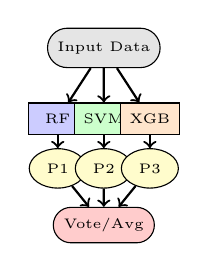
\begin{tikzpicture}[scale=0.9, every node/.style={font=\tiny}]
      % Input data
      \node[draw, fill=gray!20, rounded rectangle, minimum width=1.2cm, minimum height=0.5cm] (input) at (0.8, 2.5) {Input Data};

      % Three models
      \node[draw, fill=blue!20, rectangle, minimum width=0.75cm, minimum height=0.4cm] (m1) at (0.15, 1.5) {RF};
      \node[draw, fill=green!20, rectangle, minimum width=0.75cm, minimum height=0.4cm] (m2) at (0.8, 1.5) {SVM};
      \node[draw, fill=orange!20, rectangle, minimum width=0.75cm, minimum height=0.4cm] (m3) at (1.45, 1.5) {XGB};

      % Predictions
      \node[draw, fill=yellow!20, ellipse, minimum width=0.6cm, minimum height=0.35cm] (p1) at (0.15, 0.8) {P1};
      \node[draw, fill=yellow!20, ellipse, minimum width=0.6cm, minimum height=0.35cm] (p2) at (0.8, 0.8) {P2};
      \node[draw, fill=yellow!20, ellipse, minimum width=0.6cm, minimum height=0.35cm] (p3) at (1.45, 0.8) {P3};

      % Aggregation
      \node[draw, fill=red!20, rounded rectangle, minimum width=1cm, minimum height=0.45cm] (agg) at (0.8, 0) {Vote/Avg};

      % Arrows
      \draw[->, thick] (input) -- (m1);
      \draw[->, thick] (input) -- (m2);
      \draw[->, thick] (input) -- (m3);
      \draw[->, thick] (m1) -- (p1);
      \draw[->, thick] (m2) -- (p2);
      \draw[->, thick] (m3) -- (p3);
      \draw[->, thick] (p1) -- (agg);
      \draw[->, thick] (p2) -- (agg);
      \draw[->, thick] (p3) -- (agg);
    \end{tikzpicture}

    \iqbsep
    Reduces variance, improves robustness
  }{
    \iqbsectiontitle{Methods}
    \small
    \begin{iqbitemize}
      \item[Voting] Average (regression) or majority vote
      \item[Bagging] Random Forest, ExtraTrees
      \item[Boosting] AdaBoost, GBM, XGBoost
    \end{iqbitemize}

    \iqbsep

    \iqbsectiontitle{Stacking}
    \small
    \begin{iqbitemize}
      \item Train base learners
      \item Meta-features on validation
      \item Meta-learner (logistic regression)
      \item Final test prediction
    \end{iqbitemize}
  }
\end{frame}

% ------------------------------------------------------------
% 19. Applicability domain
% ------------------------------------------------------------
\begin{frame}{Applicability Domain (AD) Assessment}
  \iqblayouttwo{
    \iqbsectiontitle{AD techniques}
    \begin{iqbitemize}
      \item Distance-based (kNN, Mahalanobis, leverage).
      \item Probability density (Gaussian mixture, kernel density).
      \item Ensemble disagreement or variance of predictions.
    \end{iqbitemize}
  }{
    \iqbsectiontitle{Communicating AD}
    \begin{iqbitemize}
      \item Provide AD score per prediction (traffic light labels).
      \item Visualize in descriptor space; show where external compounds sit.
      \item Case study: illustrate experimental failures when AD ignored.
    \end{iqbitemize}
  }
\end{frame}
 
% ------------------------------------------------------------
% 20. Randomization tests - RESTORED AND FIXED
% ------------------------------------------------------------
% \begin{frame}{Randomization \& Robustness Tests}
%   \iqblayouttwo{
%     \iqbsectiontitle{Y-scrambling}
%     \begin{iqbitemize}
%       \item Shuffle endpoints, rebuild models; expect low \(Q^2\)/\(R^2\) if real signal exists.
%       \item Perform multiple iterations (e.g., 50-100) and plot distribution.
%     \end{iqbitemize}
%     \iqbsep
%     \iqbsectiontitle{X-scrambling / progressive scrambling}
%     \begin{iqbitemize}
%       \item Randomize descriptors gradually to assess sensitivity.
%       \item Helps detect over-dependence on a few variables.
%     \end{iqbitemize}
%   }{
%     \iqbgreenbox{Reporting tips}{
%       Document protocol (random seeds, sample size), include comparison charts, and tie back to OECD P4 robustness narrative.
%     }  % ← FIXED: Added missing closing brace
% \end{frame}

% ------------------------------------------------------------
% Part 6: Interpretation
% ------------------------------------------------------------
\iqbsectionframe{Interpretation}{模型解释}

% ------------------------------------------------------------
% 21. Global interpretation
% ------------------------------------------------------------
% Frame F1: Feature Selection & Dimensionality Reduction
\begin{frame}{Feature Selection: Curse of Dimensionality}
  \iqblayouttwo{
    \iqbsectiontitle{Why select features?}
    \begin{iqbitemize}
      \item \textbf{Many descriptors:} 5000+ (Dragon) vs. few compounds ($N < 100$) $\Rightarrow$ overfitting
      \item \textbf{Redundancy:} logP, TPSA often correlated
      \item \textbf{Interpretability:} Simpler models are more trustworthy
      \item \textbf{Cost:} Fewer descriptors to compute = faster screening
    \end{iqbitemize}

    \iqbsep

    \iqbgreenbox{Rule of thumb}{
      Aim for $N_{features} < N_{compounds} / 5$ to reduce overfitting risk
    }
  }{
    \iqbsectiontitle{Common strategies}
    \small
    \begin{iqbitemize}
      \item[Filter] Correlation-based, variance threshold, statistical test (ANOVA)
      \item[Wrapper] Forward/backward selection, recursive elimination (RFE), genetic algorithms
      \item[Embedded] L1 regularization (Lasso), tree feature importance
    \end{iqbitemize}
  }
\end{frame}

% Frame F2: Dimensionality Reduction (PCA, Autoencoders)
\begin{frame}{Dimensionality Reduction: Latent Space Exploration}
  \iqblayouttwo{
    \iqbsectiontitle{PCA}
    Linear projection; preserve $>90\%$ variance in 3--10 PCs.

    \iqbsep

    \iqbbluebox{Pros}{Interpretable; fast}

    \iqbsep

    \iqborangebox{Cons}{Loses nonlinearity}

    \iqbsep

    \iqbsectiontitle{t-SNE / UMAP}
    Nonlinear for visualization; not for modeling.
  }{
    \iqbsectiontitle{Autoencoders}
    Bottleneck learns compression. Variational (VAE) for generation.

    \iqbsep

    \iqbgreenbox{When}{$N > 1k$; GPU needed}
  }
\end{frame}

\begin{frame}{Global Interpretation: Feature Importance}
  \iqblayouttwo{
    \iqbsectiontitle{Computing importance}
    \small
    \textbf{Linear:} Coefficients magnitude

    \textbf{Tree-based:} Impurity, permutation, SHAP

    \textbf{Validation:} CV fold stability

    \textbf{Insight:} Mechanistic clues from descriptors
  }{
    \iqbimgcenter[width=0.9\textwidth]{images/qsar-ml-chap6/6.9.png}
    \iqbsep
    \centering
    \small
    Fig. 6.9: Feature importance scores.
  }
\end{frame}

% ------------------------------------------------------------
% 22. Local interpretation
% ------------------------------------------------------------
\begin{frame}{Local Interpretation: LIME and SHAP}
  \iqbsectiontitle{LIME: Local Interpretable Model-agnostic Explanations}

  \begin{center}
  % \begin{tikzpicture}[scale=0.85, every node/.style={font=\tiny}]
  %   % Step 1: Original Prediction
  %   \node[draw, fill=blue!20, rounded rectangle, minimum width=1.4cm, minimum height=0.7cm] (step1) at (0, 1.5) {Original\\Prediction};
  %   \draw[->, thick] (step1) -- (1.0, 1.5);

  %   % Step 2: Local Perturbations
  %   \node[draw, fill=green!20, rounded rectangle, minimum width=1.4cm, minimum height=0.7cm] (step2) at (2.0, 1.5) {Local\\Perturbations};
  %   \draw[->, thick] (step2) -- (3.0, 1.5);

  %   % Step 3: Predict Perturbed
  %   \node[draw, fill=yellow!20, rounded rectangle, minimum width=1.4cm, minimum height=0.7cm] (step3) at (4.0, 1.5) {Predict\\Perturbed};
  %   \draw[->, thick] (step3) -- (5.0, 1.5);

  %   % Step 4: Fit Surrogate
  %   \node[draw, fill=purple!20, rounded rectangle, minimum width=1.4cm, minimum height=0.7cm] (step4) at (6.0, 1.5) {Fit\\Surrogate};
  %   \draw[->, thick] (step4) -- (7.0, 1.5);

  %   % Step 5: Feature Importance
  %   \node[draw, fill=red!20, rounded rectangle, minimum width=1.4cm, minimum height=0.7cm] (step5) at (8.0, 1.5) {Feature\\Importance};

  %   % Explanations below
  %   \node[below=0.6cm of step2, align=center, text width=2.2cm, font=\tiny] {Perturb \& weight samples};
  %   \node[below=0.6cm of step4, align=center, text width=2.2cm, font=\tiny] {Linear surrogate fit};
  % \end{tikzpicture}
  \end{center}

  \iqbsep

  \small
  \textbf{\textcolor{blue}{LIME:}} Model-agnostic; local explanations; interactive demos; lightweight.

  \textbf{\textcolor{purple}{SHAP:}} Game theory based; consistent importance; multiple visualizations; global explanations.
\end{frame}

% ------------------------------------------------------------
% Frame B3: LIME vs. SHAP Deep Dive
% ------------------------------------------------------------
\begin{frame}{LIME vs. SHAP: Interpretability Trade-offs}
  \small
  \begin{tabular}{|l|cc|}
    \hline
    \textbf{Aspect} & \textbf{LIME} & \textbf{SHAP (Shapley Values)} \\
    \hline
    \textbf{Theoretical foundation} & Local linear approx. & Game theory \\
    \textbf{Stability} & Variable; data-dependent & Guaranteed consistent \\
    \textbf{Computation speed} & Fast (single instance) & Slow (exponential in features) \\
    \textbf{Feature interactions} & Implicit & Explicit via interaction plots \\
    \textbf{Global vs. local} & Single-instance & Can aggregate for global \\
    \textbf{Model agnostic?} & Yes & Mostly (deep learning harder) \\
    \textbf{Visualization} & Bar charts & Force plots, beeswarms, waterfall \\
    \textbf{Classroom appeal} & High; intuitive & High; theoretically sound \\
    \hline
  \end{tabular}

  \iqbsep

  \iqbgreenbox{Practical Note}{
    Use LIME for rapid prototyping and interactive demos. Switch to SHAP TreeExplainer for tree-based models (RF, XGBoost) or approximate Shapley (e.g., TreeSHAP, KernelSHAP) for deep neural networks.
  }
\end{frame}

% ------------------------------------------------------------
% Part 7: Practice & Cases
% ------------------------------------------------------------
\iqbsectionframe{Practice and Cases}{实践与案例}

% ------------------------------------------------------------
% 23. Practical checklist
% ------------------------------------------------------------
\begin{frame}{QSAR Modeling Practical Checklist}
  \iqblayouttwo{
    \iqbsectiontitle{Data readiness}
    \begin{iqbitemize}
      \item Is assay metadata complete? Units aligned?
      \item Are structures standardized (charges, salts, stereochemistry)?
      \item Are duplicates, inconclusive labels, or outliers handled?
    \end{iqbitemize}
    \iqbsep
    \iqbsectiontitle{Modeling choices}
    \begin{iqbitemize}
      \item Which representation aligns with mechanism hypotheses?
      \item What baseline models will you compare?
      \item How will you tune hyperparameters without leaking test data?
    \end{iqbitemize}
  }{
    \iqbsectiontitle{Validation \& deployment}
    \begin{iqbitemize}
      \item External set defined? AD strategy ready?
      \item Interpretability plan (global + local) documented?
      \item Deployment hooks: batch scoring, alerting on AD violations.
    \end{iqbitemize}
  }
\end{frame}

% ------------------------------------------------------------
% 24. Case studies
% ------------------------------------------------------------
% Frame B4: QSAR Variants Beyond Activity Prediction
\begin{frame}{Beyond Activity: QSAR Variants (QSPR, QSRR, QSTR)}
  \small
  \iqblayouttwo{
    \iqbsectiontitle{QSPR (Property)}
    Predict physicochemical/ADME properties from structure:
    \begin{iqbitemize}
      \item logP (lipophilicity)
      \item TPSA, H-bond donors/acceptors
      \item Aqueous solubility (logS)
      \item Metabolic stability (microsomal T$_{1/2}$)
    \end{iqbitemize}

    \iqbsep

    \iqbgreenbox{Challenge}{
      Properties often continuous and unbounded; require larger datasets for robust models.
    }
  }{
    \iqbsectiontitle{QSRR \& QSTR}
    \begin{iqbitemize}
      \item[QSRR] Predict reaction rate or kinetics; rate constants, activation energies, selectivity
      \item[QSTR] Toxicity risk; acute LD$_{50}$ predictions, carcinogenicity/mutagenicity flags, regulatory QSAR
    \end{iqbitemize}
  }
\end{frame}

% Frame C1: Graph Neural Networks (GNN) for QSAR
\begin{frame}{GNNs \& Molecular Graphs: Next-Generation QSAR}
  \iqblayoutthree{
    \iqbsectiontitle{Why Graphs?}
    \small
    \begin{iqbitemize}
      \item Preserve topology; encode atoms \& bonds directly
      \item Permutation invariant; no manual alignment
      \item Scalable to large libraries
      \item Support multi-task learning
    \end{iqbitemize}
  }{
    \iqbsectiontitle{Common Architectures}
    \small
    \begin{iqbitemize}
      \item[GraphConv] Simple graph convolution
      \item[Chemprop] D-MPNN; message passing from bond features
      \item[AttentiveFP] Attention layers; interpretable edge/atom weights
      \item[GIN] Graph Isomorphism Network
    \end{iqbitemize}
  }{
    \iqbsectiontitle{In Practice}
    \small
    \begin{iqbitemize}
      \item Outperform traditional descriptors on large datasets ($N > 5k$)
      \item Transfer learning: pre-train on big pharma data
      \item Challenge: black-box; need LIME/SHAP for explanation
    \end{iqbitemize}

    \iqbsep

    \textbf{Tools:} RDKit, PyTorch Geometric, Chemprop
  }
\end{frame}

\begin{frame}{2023-2024 Success Stories}
  \iqblayouttwo{
    \iqbsectiontitle{Highlighted applications}
    \begin{iqbitemize}
      \item Anti-parasitic leads: QSAR + Chemprop-guided synthesis for \textit{T. cruzi}.
      \item IL-2 modulation: multi-task QSAR finds dual-activity scaffolds.
      \item \textit{S. aureus} antibacterial screens with ML-prioritized libraries.
    \end{iqbitemize}
  }{
    \iqbsectiontitle{Process themes}
    \begin{iqbitemize}
      \item Closed experimental loops confirm in-silico predictions.
      \item Platform examples: PhaKinPro for ADME predictions, industrial Chemprop deployments.
      \item Stress reproducibility: public code releases + benchmark datasets.
    \end{iqbitemize}
  }
\end{frame}

% ------------------------------------------------------------
% Part 8: Outlook & Summary
% ------------------------------------------------------------
\iqbsectionframe{Outlook and Summary}{展望与总结}

% ------------------------------------------------------------
% 25. Challenges
% ------------------------------------------------------------
\begin{frame}{Challenges \& Future Directions}
  \iqblayouttwo{
    \iqbsectiontitle{Current pain points}
    \begin{iqbitemize}
      \item Cross-lab variability and incomplete metadata.
      \item Class imbalance, bias reporting, and uncertainty quantification.
      \item Limited mechanistic insight for black-box DL.
    \end{iqbitemize}
  }{
    \iqbsectiontitle{Opportunities}
    \begin{iqbitemize}
      \item Multi-task, transfer, and federated learning for data-scarce targets.
      \item Integration with knowledge graphs and causal modeling.
      \item Automated data governance + audit trails for OECD compliance at scale.
    \end{iqbitemize}
  }
\end{frame}

% ------------------------------------------------------------
% 26. Summary
% ------------------------------------------------------------
\begin{frame}{Summary \& Next Steps}
  \iqbbluebox{Key takeaways}{
    \begin{iqbitemize}
      \item QSAR links chemical structure to activity; success hinges on curated data and thoughtful representations.
      \item OECD principles offer a checklist for credible, regulator-ready models.
      \item Validation, applicability domain, and interpretation must be planned alongside modeling.
      \item Modern ML and GNNs expand predictive power but magnify the need for transparency and governance.
    \end{iqbitemize}
  }

  \iqbsep

  \iqbgreenbox{For the classroom}{
    Conclude with a mini-quiz (identify OECD principle given a scenario) or assign students to map a project proposal onto the practical checklist.
  }
\end{frame}

\end{document}

